\documentclass[12pt]{article}
\usepackage[T1]{fontenc}
\usepackage[top=2.5cm, bottom=2.5cm, left=3cm, right=2.5cm]{geometry}
\usepackage{setspace}
\usepackage{graphicx}
\usepackage{amsmath}
\usepackage{amssymb}
\usepackage{braket}
\usepackage{cite}
\usepackage{tikz}
\usetikzlibrary{positioning,calc,fit,shapes.geometric,arrows.meta}
\usepackage{quantikz}
\usepackage{booktabs}
\usepackage{float}
\usepackage{subcaption}
\usepackage[hidelinks]{hyperref}
\usepackage{fancyhdr}
\usepackage{titlesec}
\titleformat{\section}{\LARGE\bfseries}{\thesection}{1em}{}
\titleformat{\subsection}{\large\bfseries}{\thesubsection}{1em}{}
\titleformat{\subsubsection}{\normalsize\bfseries}{\thesubsubsection}{1em}{}

\pagestyle{fancy}
\fancyhf{}
\fancyhead[L]{\small\itshape Beyond Prepare-and-Measure}
\fancyhead[R]{\small\itshape Linus Kelsey}
\fancyfoot[C]{\thepage}
\renewcommand{\headrulewidth}{0.4pt}
\renewcommand{\footrulewidth}{0pt}

\let\oldsection\section
\renewcommand{\section}{\clearpage\oldsection}

\title{Beyond Prepare-and-Measure: The Cost of Trustless Detectors in Quantum Key Distribution}
\author{Linus Kelsey}
\date{Aug 2026}

\begin{document}
\onehalfspacing
\maketitle
\thispagestyle{empty}

\begin{abstract}
Quantum Key Distribution (QKD) was first put forward in 1984 by Bennett and Brassard through their foundational proposal for bipartite secure key exchange taking advantage of quantum mechanics, now commonly known as BB84. In the following decades, a number of inspired methods have emerged to guarantee shared secrecy. In particular, Measurement-Device-Independent (MDI) QKD, presented in 2012, improves BB84 security assumptions by eliminating the need to trust photon detectors. In order to be able to deploy QKD at scale, providers must map the trade-offs of either protocol, and comparisons of the two in secure information exchange rate (key rate), cost and scalability allow for efficient application of this maturing technology. In this report, we aim to contribute to the solution of this problem through use of NetSquid, a quantum network discrete event simulation (DES) engine, and an algebraic cost model, to simulate and compare network behaviour for both MDI-QKD and BB84. We see that the price to pay for MDI's improved security is a drop in key rate, of up to 10 times, in modest metropolitan networks under realistic hardware assumptions.
\end{abstract}

\newpage
\tableofcontents
\thispagestyle{plain}
\newpage

\section{Introduction}

The advent of large-scale quantum computing poses a fundamental threat to classical public-key cryptography. Modern key-exchange standards, including RSA \cite{RSA_1978} and Elliptic Curve Cryptography \cite{Koblitz_ECC,Miller_ECC}, derive their security from the computational hardness of integer factorisation and the discrete logarithm problem. Shor's algorithm \cite{Shor_1997}, published in 1997, demonstrated that both problems can be solved in polynomial time on a sufficiently powerful quantum computer, rendering these standards vulnerable to a quantum-capable adversary. Post-Quantum Cryptography (PQC) responds to this threat by identifying classically hard problems not susceptible to known quantum speed-ups; Quantum Key Distribution (QKD) takes the complementary route, using quantum mechanics to guarantee shared secrecy rather than computational assumption.

QKD was first conceived by Wiesner \cite{Wiesner_1983} in the 1970s and given its first operational form by Bennett and Brassard in 1984 \cite{Bennett_2014}. In the decades since, QKD has matured into one of the most field-tested quantum technologies, with national-scale fibre deployments serving over 150 users across thousands of kilometres \cite{chen2021} and metropolitan testbeds demonstrating sustained multi-vendor operation \cite{Peev_2009,Sasaki_2011}. This trajectory has motivated a growing body of research into how QKD protocols should be chosen and deployed at scale. This work focuses on two protocols that represent a natural axis of comparison: BB84, the original Prepare-and-Measure scheme, and Measurement-Device-Independent QKD (MDI-QKD), proposed by Lo, Curty and Qi in 2012 \cite{Lo_2012}. Their protocols and theoretical performance bounds are introduced in Section~\ref{sec:background}.

MDI-QKD improves upon BB84's security model by removing the need to trust photon detectors, an assumption that is difficult to verify in practice and has been exploited in hardware-level attacks. This advantage, however, comes at a real cost in key rate: at metropolitan distances, BB84 consistently delivers rates an order of magnitude higher than MDI under comparable hardware conditions \cite{Dynes_2019,Yan2025}. For network providers selecting between the two protocols, this trade-off must be mapped carefully across distance, topology, and network scale. The question is not simply which protocol is more secure, but under what deployment conditions MDI's security advantage justifies its rate penalty, and at what economic and energetic cost.

Despite the commercial momentum behind both protocols — evidenced by a progression of field deployments from early national testbeds \cite{Elliott_2002,Peev_2009,Sasaki_2011,chen2021,Qin_NQSN_2024} through metropolitan and long-haul fibre networks \cite{Dynes_2019,pittaluga_2024} to dedicated MDI-QKD systems \cite{Tang_2016,Berrevoets_2022,qbird_belQCI}, heterogeneous multi-vendor network trials \cite{Martins2024}, and European infrastructure programmes \cite{eu_open_qkd} — the quantitative basis for choosing between BB84 and MDI-QKD for a given application remains poorly characterised. Simulation of MDI-QKD at metropolitan scale has not systematically explored the interplay between topology, relay placement, and hardware parameters across a sufficiently wide parameter space to support confident protocol selection \cite{Yehia_2022}. Cost models for MDI networks are largely absent from the literature: whilst integer linear programming approaches have been developed for PM and entanglement-based QKD infrastructure \cite{DBLP:conf/ondm/KaraviasHBLP25}, their extension to MDI has not been carried out. Energetic footprint, an increasingly central criterion in telecommunications infrastructure procurement, has only recently begun to receive attention in the QKD context \cite{Yehia_2025}. A rigorous parametric comparison across key rate, cost, and scalability is absent.

This work addresses these gaps through a two-part methodology. First, we implement and simulate both protocols within NetSquid \cite{Coopmans_2021}, a discrete-event quantum network simulation engine, across a ten-layer hardware model spanning ideal to physically realistic conditions. Second, we derive deployment cost formulae algebraically using symbolic per-component parameters---cost per photon source $c_s$, per single-photon detector $c_d$, and per km of installed dark fibre $c_f$---expressing each protocol's total infrastructure cost as a closed-form function of user count and topology. Since manufacturer prices for quantum dot sources and single-photon detectors are not publicly available, absolute CapEx comparison is deferred to the parameter space; the structural scaling difference between protocols is the primary analytical result. We compare BB84 and MDI-QKD across three dimensions: key rate as a function of distance and hardware parameters; relative deployment cost as a function of network size; and scalability, defined as the marginal key rate when adding users to a fixed metropolitan topology. The remainder of this report is structured as follows. Section~\ref{sec:background} introduces the protocols, their hardware underpinnings, and the theoretical performance bounds that govern them. Section~\ref{sec:methodology} describes the simulation architecture and cost model. Section~\ref{sec:results} presents results across all three comparison axes, and Section~\ref{sec:conclusion} concludes with deployment recommendations and directions for future work.

\section{Shared Quantum Secrecy}
\label{sec:background}

Quantum Key Distribution refers to any communications protocol in which two or more parties use quantum channels, the sharing of quantum states, together with authenticated classical channels and post-processing, to establish a shared secret cryptographic key. The security of such a scheme is guaranteed by the laws of quantum mechanics, providing information-theoretic security against any eavesdropper whose capabilities are bounded by quantum physics. Since Bennett and Brassard's foundational paper in 1984 \cite{Bennett_2014}, numerous variants of QKD have been proposed. This work focuses on two: the original Prepare-and-Measure scheme (BB84) and Measurement-Device-Independent QKD (MDI-QKD), proposed by Lo, Curty and Qi in 2012 \cite{Lo_2012}.

\subsection{BB84}

BB84 is representative of the class of Prepare-and-Measure (PM) protocols. Alice begins by preparing a string of $n$ photons, each encoded in one of four polarisation states ($0^\circ$, $45^\circ$, $90^\circ$ or $135^\circ$) selected uniformly at random. In the qubit formalism, these correspond to $\ket{0}$, $\ket{+} = \tfrac{1}{\sqrt{2}}(\ket{0}+\ket{1})$, $\ket{1}$ and $\ket{-} = \tfrac{1}{\sqrt{2}}(\ket{0}-\ket{1})$, respectively. Alice selects a basis ($\{\ket{0},\ket{1}\}$ or $\{\ket{+},\ket{-}\}$) for each qubit uniformly and independently, then uniformly and independently again, she applies a bit flip within that basis before transmission.

She transmits these quantum states to Bob over a quantum channel. Bob measures each photon in a uniformly and independently random basis. Alice and Bob then use an authenticated classical channel to compare basis choices and discard all photons measured in mismatching bases, producing a raw, sifted key. A portion of this sifted key is compared over the classical channel to estimate the Quantum Bit Error Rate (QBER): the fraction of photon pairs measured in the same basis that nevertheless disagree. A QBER below $11\%$ is taken as evidence that the channel has not been compromised \cite{Shor_2000}. Alice and Bob then apply error correction and privacy amplification (hash-based post-processing that shortens the raw key, removing any partial information an eavesdropper may have gathered) to produce the final shared secret key. Figure~\ref{fig:bb84_comm} illustrates the basic bipartite logical layer.

\begin{figure}[H]
    \centering
    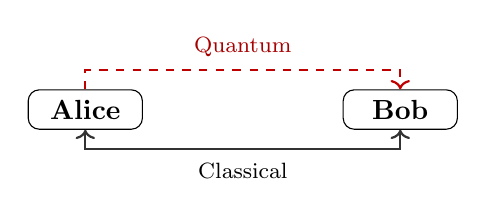
\begin{tikzpicture}
        \tikzset{
            party/.style={draw, rounded corners, minimum width=1.45cm, minimum height=0.5cm, align=center, font=\bfseries},
            qcomm/.style={red!75!black, dashed, thick},
            ccomm/.style={black!60!gray, thick}
        }
        \node[party] (A) at (-2,0) {Alice};
        \node[party] (B) at (2,0) {Bob};
        \node[] (J) at (0, 0.5) {};
        \node[above=5pt of J.south, font=\footnotesize, align=center, red!65!black] {Quantum};
        \node[] (K) at (0, -0.5) {};
        \node[below=5pt of K.north, font=\footnotesize, align=center] {Classical};
        \draw[-,qcomm] (A.north) |- (J);
        \draw[->,qcomm] (J.west) -| (B.north);
        \draw[->,ccomm] (K.west) -| (A.south);
        \draw[->,ccomm] (K.west) -| (B.south);
    \end{tikzpicture}
    \caption{Communication diagram for point-to-point BB84. Alice sends quantum states to Bob; basis reconciliation and post-processing occur over authenticated classical channels.}
    \label{fig:bb84_comm}
\end{figure}

Security proofs for BB84, and QKD generally, are conditional on the modelling assumptions made about devices, network, and attacker capabilities. A particular vulnerability in practice arises from weak coherent pulse (WCP) laser sources, whose photon number per pulse follows a Poisson distribution. Multi-photon pulses allow a Photon Number Splitting (PNS) attack \cite{PNS_desc}, in which Eve intercepts and holds trailing photons until bases are announced, extracting key information without disturbing the QBER. The decoy-state technique \cite{Lo_decoys} mitigates this by varying pulse intensity randomly, enabling Alice and Bob to tightly bound the single-photon contribution to their key.

\subsection{Measurement-Device-Independent QKD}

MDI-QKD addresses a fundamental vulnerability shared by all PM schemes: the need to trust the measurement devices at Bob's node. Side-channel attacks on detectors represent a significant practical threat, as the gap between idealised device models assumed in security proofs and real hardware is difficult to close. MDI removes detectors entirely from the trust boundary by introducing an untrusted third-party relay, Charlie, who performs all measurement operations.

In MDI-QKD, both Alice and Bob independently prepare photon strings in the manner of BB84 and transmit these to Charlie. Charlie performs a Bell State Measurement (BSM) on each arriving photon pair, projecting onto the two-qubit Bell basis:
\[
    \ket{\phi^\pm} = \frac{\ket{00} \pm \ket{11}}{\sqrt{2}}, \qquad \ket{\psi^\pm} = \frac{\ket{01} \pm \ket{10}}{\sqrt{2}}.
\]
Charlie announces the measurement outcome over a classical channel to both Alice and Bob. Since the BSM measures only the \emph{joint correlation} between the two incoming photons rather than their individual polarisations, an eavesdropper with full control of Charlie's apparatus can learn nothing about Alice's or Bob's individual bit values. The physical mechanism underlying the BSM is Hong-Ou-Mandel (HOM) interference~\cite{Hong_1987}: two indistinguishable photons arriving simultaneously at a 50:50 beam splitter always exit the same output port due to bosonic quantum interference. Coincident clicks at the downstream polarising beam splitters then identify the projected Bell state. Photon indistinguishability is therefore a prerequisite for MDI-QKD: timing jitter, spectral mismatch, and polarisation misalignment all reduce HOM visibility and degrade BSM success probability. The bipartite logical layer for MDI-QKD is shown in Figure~\ref{fig:mdi_comm}.

\begin{figure}[H]
    \centering
    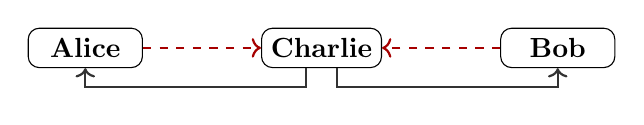
\begin{tikzpicture}
        \tikzset{
            party/.style={draw, rounded corners, minimum width=1.45cm, minimum height=0.5cm, align=center, font=\bfseries},
            qcomm/.style={red!65!black, dashed, thick},
            ccomm/.style={black!60!gray, thick}
        }
        \node[party] (A) at (-3,0) {Alice};
        \node[party] (B) at (3,0) {Bob};
        \node[party] (C) at (0,0) {Charlie};
        \draw[->,qcomm] (A.east) -- (C.west);
        \draw[->,qcomm] (B.west) -- (C.east);
        \node[] (J) at (-1.5,-0.5) {};
        \node[] (K) at (1.5,-0.5) {};
        \draw[-,ccomm] ($(C.south)+(-0.2,0)$) |- (J.west);
        \draw[-,ccomm] ($(C.south)+(0.2,0)$) |- (K.east);
        \draw[->,ccomm] (J) -| (A.south);
        \draw[->,ccomm] (K) -| (B.south);
    \end{tikzpicture}
    \caption{Communication diagram for point-to-point MDI-QKD. Both Alice and Bob transmit quantum states to Charlie; Charlie performs a BSM and announces the result classically to both parties.}
    \label{fig:mdi_comm}
\end{figure}

Alice and Bob sift by matching bases as in BB84. Upon receiving the BSM outcome, each party knows their own basis choice and bit value, and can deduce the other's bit via the outcome. Depending on the Bell state announced, one party selectively bit-flips to ensure agreement, as summarised in Table~\ref{tab:mdi_flips}. In the linear-optical BSM implementation, only two of the four Bell states ($\ket{\psi^+}$ and $\ket{\psi^-}$) are unambiguously distinguishable \cite{Lo_2012}; detection events corresponding to $\ket{\phi^\pm}$ are discarded as inconclusive. Privacy amplification and error correction then proceed as in BB84.

\begin{table}[H]
    \centering
    \begin{tabular}{lcc}
        \toprule
        BSM outcome & $\ket{\psi^{+}}$ & $\ket{\psi^{-}}$ \\
        \midrule
        Diagonal basis    & No bit flip & Bit flip \\
        Rectilinear basis & Bit flip    & Bit flip \\
        \bottomrule
    \end{tabular}
    \caption{Bit-flip rules upon receipt of BSM outcome~\cite{Lo_2012}. Alice and Bob agree in advance which party applies the flip; if both flip, there is no net change.}
    \label{tab:mdi_flips}
\end{table}

The abstract operation of the BSM in quantum information terms is shown in Figure~\ref{fig:bsm_circ}: a CNOT gate followed by a Hadamard and measurement. The physical implementation uses a 50:50 beam-splitter and polarising beam-splitters, with the Hong-Ou-Mandel effect ensuring that only coincidence detection events, two simultaneous clicks at the detector array, constitute valid BSM outcomes.

\begin{figure}[H]
    \centering
    \begin{quantikz}
        \lstick{$q_0$} & \ctrl{1} & \gate{H} & \meter{} \\
        \lstick{$q_1$} & \targ{}  &          & \meter{}
    \end{quantikz}
    \caption{Bell State Measurement circuit: CNOT gate followed by Hadamard, then measurement in the computational basis.}
    \label{fig:bsm_circ}
\end{figure}

MDI-QKD's security advantage comes at a cost. Key generation requires a successful coincidence detection at Charlie -- both photons from Alice and Bob must arrive and be detected within the same time window. This requirement, combined with independent connection losses on each arm, imposes a rate penalty relative to BB84's single-link loss \cite{Lo_2012}. MDI's QBER tolerance is also more sensitive than BB84's, as two independent quantum channels each contribute noise, enlarging the attack surface accounted for by security proofs.

\subsection{Theoretical Performance Bounds}

The maximum achievable secure key rate in any point-to-point (no quantum repeater) QKD scheme is bounded by the Pirandola--Laurenza--Ottaviani--Banchi (PLOB) bound \cite{Pirandola_2017}. This fundamental result establishes that, against all attacks permitted by quantum physics, the key rate of a repeater-less link scales at most linearly with channel transmittance $\eta$:
\[
    R \leq -\log_2(1 - \eta) \approx \eta \log_2 e \quad \text{for } \eta \ll 1.
\]
Since transmittance decays exponentially with fibre length $L$ as $\eta = 10^{-\alpha L / 10}$ (with $\alpha$ the fibre attenuation coefficient in dB/km), the PLOB bound implies that key rates must fall exponentially with distance. Both BB84 and standard MDI-QKD are subject to this bound.

Twin-Field QKD (TF-QKD), proposed in 2018 by Lucamarini et al.\ \cite{Lucamarini_2018}, exploits the same untrusted-relay tenet as MDI but replaces the two-photon BSM with single-photon interference. The result is that key rates scale as $\mathcal{O}(\sqrt{\eta})$ rather than $\mathcal{O}(\eta)$, exceeding the PLOB bound and extending the distance at which secure communication is achievable. TF-QKD thus represents the most practically significant near-term stepping stone beyond the repeater-less limit, and motivates the question central to this work, of precisely where and under what conditions MDI-QKD's security advantage over BB84 justifies its rate penalty, before that regime is superseded by TF-QKD or, eventually, quantum repeaters.

\subsection{Network Topologies}
\label{sec:network_topologies}

When QKD is deployed beyond a single point-to-point link, network topology becomes a primary driver of cost and scalability. BB84 requires a dedicated quantum channel between every pair of users: for $N$ users, a full mesh demands $\binom{N}{2} = \mathcal{O}(N^2)$ fibre spans, each carrying an independent quantum signal. MDI-QKD's architecture naturally admits a star topology instead: all users direct their pulses to a shared measurement node (Charlie), which performs the Bell-state measurement without accessing the key material. Crucially, Charlie need not be trusted---the measurement-device-independence property is preserved at network scale, so the relay introduces no new security assumption. For $K$ relay nodes each serving a cluster of users, the MDI network requires $\mathcal{O}(N)$ user--relay fibre spans and $\mathcal{O}(K^2)$ inter-relay backbone links, both substantially below the $\mathcal{O}(N^2)$ full mesh for $K\ll N$. This structural asymmetry---summarised in the component-count model of Section~\ref{sec:cost_model}---is the central economic and scalability argument evaluated in this work.

\section{Methodology}
\label{sec:methodology}
We compare BB84 and MDI-QKD across three dimensions: performance, deployment cost, and scalability. Together these axes capture the trade-off a network provider faces when selecting between the two protocols for a given metropolitan deployment.

\textit{Performance.} The primary metric is secure key rate, measured in bits per second: the length of the final distilled key divided by the time taken to produce it. Since all QKD-generated keys are information-theoretically equivalent in security regardless of protocol, key rate is the sole performance discriminant between BB84 and MDI-QKD. We simulate key rate as a function of distance and individual hardware parameters using NetSquid \cite{Coopmans_2021}, a discrete-event quantum network simulation engine, across a ten-layer hardware model that progressively introduces realistic physical imperfections from an ideal baseline.

\textit{Cost.} Deployment cost is modelled algebraically using symbolic per-component parameters: $c_s$ (photon source), $c_d$ (single-photon detector), and $c_f$ (fibre per km). The number of each component is determined by the network topology under each protocol. Since manufacturer prices for quantum dot sources and single-photon detectors are not publicly available at the precision required for quantitative comparison, we express total cost symbolically and focus on the \textit{relative} cost structure between protocols. This reveals a structural crossover: BB84 fibre cost scales as $\mathcal{O}(N^2)$ whilst MDI scales as $\mathcal{O}(N)$ at fixed relay count $K$, so MDI becomes cost-competitive above a threshold user count $N^*$ whose value depends on the ratio $c_d/c_f$ and network geometry.

\textit{Scalability.} We define scalability as the marginal key rate incurred when adding a user to an existing network. Since BB84 requires a direct link between every user pair whilst MDI routes traffic through relay nodes, the two protocols exhibit fundamentally different scaling behaviour. We quantify this by sweeping user count at fixed topology parameters and extracting per-user marginal key rates.

\subsection{Performance Analysis}
\label{sec:performance}

The primary performance metric is the secure key rate $R$, measured in bits per second: the key length extracted by a simulation run divided by the simulation duration. Since all QKD-generated keys are information-theoretically equivalent in security regardless of protocol, key rate is the sole performance discriminant between BB84 and MDI-QKD for a given network. A symmetric QBER threshold of 11\% is applied: simulation runs with QBER above this value are discarded as failures~\cite{Shor_2000}. All key rates are computed in the asymptotic regime, without finite-key corrections; this overestimates extractable key at low photon count rates but is standard in comparative simulation studies at metropolitan scale.

\subsubsection{NetSquid Simulation Engine}

NetSquid~\cite{Coopmans_2021} is a discrete-event simulation (DES) engine for quantum networks developed at QuTech, chosen for this work over analytical probability models and general-purpose DES tools for three reasons. First, NetSquid is purpose-built for quantum networks: it natively represents quantum states as density matrices evolved by quantum channels modelled as Kraus operator maps, providing physically accurate treatment of loss, decoherence, and measurement without hand-coding quantum mechanics. Second, the DES framework handles temporally correlated dynamics --- detector dead time, photon timing jitter, coincidence windows, entanglement distillation timeouts --- that a static i.i.d. probability model cannot accommodate; these effects become significant when extending to quantum repeater chains or adaptive protocols, and the DES infrastructure supports that extension without architectural changes. Third, NetSquid's \texttt{Protocol} abstraction allows each party's logic (photon preparation, transmission, basis announcement, sifting) to be written as an event-driven coroutine that yields at each physical event, making the simulation structure directly parallel to the protocol description in Section~\ref{sec:background} and reducing the gap between specification and implementation. As discussed in Section~\ref{sec:discussion}, the i.i.d. trial structure adopted here could in principle be reproduced analytically, but the DES overhead is justified by the extensibility it provides.

NetSquid organises a simulation into three layers of abstraction. \textit{Components} represent physical hardware: \texttt{QuantumChannel} objects carry photons between nodes, applying noise models (loss, dephasing, delay) as Kraus operators; \texttt{ClassicalChannel} objects carry classical messages for basis reconciliation and BSM announcements. \textit{Nodes} represent network parties (Alice, Bob, Charlie), each holding named ports through which components connect; nodes own their local quantum processors and memory registers. \textit{Protocols} are event-driven coroutines that run on nodes, yielding control to the DES scheduler at each \texttt{await} expression until a subscribed event fires. This three-layer structure maps directly onto the physical network: changing a component's noise model (e.g.\ swapping a lossless channel for one with $\alpha = 0.18$~dB/km) is localised to a single object and does not require protocol logic to change, supporting the ten-layer hardware sweep described in Section~\ref{sec:hardware_model}.

Each simulation trial instantiates a fresh NetSquid environment via \texttt{ns.sim\_reset()}, preventing cross-trial state contamination. Nodes are connected by \texttt{QuantumChannel} objects carrying a \texttt{DephaseNoiseModel} with per-arm dephasing probability $p_\phi = \min(1, \beta L)$ for arm length $L$~km, and a stochastic \texttt{HybridDelayModel} with mean propagation speed $0.8c$ and 5\% per-km Gaussian jitter. Photon loss is applied stochastically at the source before transmission using the combined Beer-Lambert and insertion loss transmittance $T = 10^{-\alpha L/10}(1 - L_i)$, and additionally at the receiver as a probabilistic discard with probability $1 - 10^{-\Delta_n/10}$. The simulation clock runs until classical post-processing completes or a 100-second simulation timeout is reached.

Trials are executed in parallel using Python's \texttt{multiprocessing} module with a \texttt{spawn} context. The spawn start method is required rather than fork because NetSquid maintains process-level global state that would be silently corrupted by copy-on-write fork sharing. The pool is sized to 80\% of available CPU cores by default. In the point-to-point setting, $r$ trials are batched in blocks of 100 and distributed across workers; in the network setting, one task is issued per user pair and all $N(N-1)/2$ tasks are dispatched in a single \texttt{pool.map} call. Results are aggregated in the main process and persisted to an SQLite database (\texttt{results.db}) via a dedicated library (\texttt{lib/db.py}). Two tables are maintained: \texttt{p2p\_results} stores one row per simulation trial (key rate, QBER, all physical parameters); \texttt{network\_results} stores one aggregated row per network run (mean key rate, success rate, topology parameters). This separation enables figure regeneration and post-hoc filtering without re-running simulations.

\subsubsection{Hardware Model}
\label{sec:hardware_model}

Physical impairments are introduced via a ten-layer parametric model. Each layer adds one impairment cumulatively to the previous, from a fully ideal baseline (layer~0) to a system incorporating all realistic imperfections (layer~9). This structure allows the marginal impact of each physical parameter on key rate to be isolated, forming the basis of the parameter sweep analysis in Section~\ref{sec:results}. Table~\ref{tab:layers} lists the ten layers.

\begin{table}[H]
\centering
\small
\begin{tabular}{cp{4.2cm}lp{2.8cm}p{3.5cm}}
\toprule
Layer & Parameter added & Symbol & Default value & Verification source \\
\midrule
0 & Ideal baseline & --- & All perfect & --- \\
1 & Fibre attenuation & $\alpha$ & 0.18~dB/km & Corning \cite{corning_smf28} \\
2 & Detector efficiency & $\eta_Z$ & 0.90 & ID Quantique \cite{idq_id281} \\
3 & Dark count rate & $d_c$ & 50~cps & ID Quantique \cite{idq_id281} \\
4 & TX insertion loss & $L_i$ & 0.10 (10\%) & \\
5 & RX node loss & $\Delta_n$ & 2.0~dB & \\
6 & Source error rate & $\varepsilon_s$ & 0.015 & Quandela \cite{QuandelaSPS} \\
7 & Fibre dephasing & $\beta$ & $10^{-4}$~ns$^{-1}$ & \\
8 & X-basis detector bias & $\eta_X$ & 0.85 & \\
9 & Beam-splitter efficiency & $\eta_\text{BS}$ & 0.97 & \\
\midrule
--- & Relay position & $\delta$ & 0.5 & User symmetry \\
\bottomrule
\end{tabular}
\caption{Ten-layer hardware model. Layer $k$ includes all impairments of layer $k-1$ plus the new parameter listed. Layer~9 is the realistic operating point used for network simulations. Empty cells in the verification column indicate parameters pending datasheet confirmation.}
\label{tab:layers}
\end{table}

\textit{Layer~0} is the ideal baseline: photons propagate without loss or noise, so key rate is limited only by propagation delay. Bipartite sweeps at this layer vary distance across the metropolitan range (0--50~km), establishing an upper bound on achievable key rate and confirming correct simulation timing before physical impairments are introduced.

\textit{Layer~1} adds fibre attenuation: each photon is discarded before transmission with probability $p_\text{loss} = 1 - 10^{-\alpha L/10}$, where $\alpha = 0.18$~dB/km and $L$ is the arm length. For MDI-QKD the two arms attenuate independently, so coincidence probability scales as the product of both arm transmittances.

\textit{Layer~2} introduces Z-basis detector efficiency $\eta_Z = 0.90$: each photon arriving at the receiver is accepted with probability $\eta_Z$. Missed detections reduce key length but do not introduce errors.

\textit{Layer~3} adds dark count rate $d_c = 50$~cps: a spurious click fires per time slot with probability $d_c / (d_c + f)$, where $f$ is the source repetition rate. Dark clicks on empty slots generate false detections; dark clicks on occupied slots override the measurement with a random bit, contributing directly to QBER.

The default detector parameters ($\eta_Z = 0.90$, $d_c = 50$~cps, layers~2--3) correspond to a superconducting nanowire single-photon detector (SNSPD) operating point, verified against the ID Quantique (IDQ) ID281~\cite{idq_id281}. The bipartite parameter sweeps in Section~\ref{sec:results_p2p} additionally span the single-photon avalanche diode (SPAD) regime ($\eta_Z \approx 0.10$--$0.25$, $d_c \approx 100$--$200$~cps), representative of the IDQ ID230~\cite{idq_id230}, covering the full range of detector technologies relevant to near-term metropolitan deployments.

\textit{Layer~4} adds TX insertion loss $L_i = 0.10$: a fixed fraction of photons is lost at the source before entering the fibre, absorbed into the combined transmittance $T = 10^{-\alpha L/10}(1 - L_i)$.

\textit{Layer~5} introduces receiver node loss $\Delta_n = 2.0$~dB as a single lumped parameter applied uniformly to both protocols, capturing the insertion loss of optical receiver components (EOM, PBS, HOM coupler). Each photon surviving fibre transmission is discarded with probability $1 - 10^{-\Delta_n/10}$ before reaching the detector. Individual component losses are not modelled separately and the protocol-specific breakdown is noted as a limitation in Section~\ref{sec:discussion}.

\textit{Layer~6} adds source error rate $\varepsilon_s = 0.015$: each emitted photon receives an unintended $\hat{X}$ flip with probability $\varepsilon_s$, modelling multi-photon emission events characterised by $g^{(2)}(0)/2$ for the reference single-photon source~\cite{QuandelaSPS}. Ideal single-photon sources are assumed throughout; WCP sources and decoy-state techniques~\cite{Lo_decoys} are not modelled, so reported rates represent an upper bound relative to practical laser deployments.

\textit{Layer~7} adds fibre dephasing $\beta = 10^{-4}$~ns$^{-1}$: the \texttt{DephaseNoiseModel} applies a per-photon dephasing error with probability $p_\phi = \min(1, \beta L)$ proportional to arm length, modelling polarisation-mode dispersion in standard single-mode fibre.

\textit{Layer~8} introduces X-basis detector bias $\eta_X = 0.85$: photons measured in the X basis are detected with lower efficiency than those in the Z basis, reflecting inter-channel efficiency variation within the same detector unit.

\textit{Layer~9} (MDI only) adds beam-splitter efficiency $\eta_\text{BS} = 0.97$: the HOM coupler at Charlie's relay has non-unit splitting ratio, reducing coincidence detection probability per arm. The relay position $\delta = 0.5$ (Charlie at the link midpoint) is held fixed for all bipartite sweeps, reflecting user symmetry; it is determined geometrically in the network setting via Equation~\ref{eq:charlie_pos}.

\subsubsection{Bipartite Single-Link Analysis}

The bipartite simulation sweeps one hardware parameter at a time, holding all others at their layer-9 defaults (Table~\ref{tab:layers}). For each parameter value, $r = 20$ independent Monte Carlo trials are run; each trial constitutes one complete QKD exchange from photon emission through key sifting. The mean key rate, mean QBER, and success rate (fraction of trials with QBER $< 11\%$) are reported as a function of the swept parameter.

\textbf{BB84 simulation.} Alice and Bob are represented as \texttt{Node} objects connected by one quantum channel (Alice $\to$ Bob) and two classical channels for basis announcement and sifting. Alice prepares $n = 1{,}024$ photons at $f = 10^7$~Hz. Each photon is assigned an independent random basis ($Z$ or $X$) and bit value. Encoding is applied qubit-by-qubit: a bit-1 value applies $\hat{X}$; an $X$-basis choice applies a Hadamard gate. Source imperfection ($\varepsilon_s$) is modelled by an additional $\hat{X}$ flip applied with probability $\varepsilon_s$, consistent with the multi-photon emission rate $g^{(2)}(0)/2$ of the reference single-photon source. Photons are discarded before transmission with probability
\begin{equation}
    p_\text{loss} = 1 - 10^{-\alpha L/10}\,(1 - L_i),
\end{equation}
modelling both fibre attenuation and TX coupling loss. The quantum channel applies an additional per-photon dephasing error of probability $\beta L$. At Bob, each arriving photon is further subject to receiver node loss (probability $1 - 10^{-\Delta_n/10}$), then detected with probability $\eta_Z$ (Z~basis) or $\eta_X$ (X~basis). Dark counts fire with per-slot probability $d_c / (d_c + f)$; a dark click on a slot where a real detection also occurs overrides with a random outcome. Dark clicks also fire on slots where the photon was lost.

After transmission, Bob announces his measurement bases and the indices of his detected slots; Alice returns her basis list. Bob retains only detections where both parties chose the same basis. The sifted key is the list of Bob's raw measurement outcomes at matching-basis slots. QBER is the fraction of bit disagreements between Alice's and Bob's sifted keys:
\begin{equation}
    \text{QBER} = \frac{1}{\ell}\sum_{k=1}^{\ell}\mathbf{1}[a_k \neq b_k],
    \label{eq:qber}
\end{equation}
where $\ell$ is the sifted key length. The QBER is measured over the full sifted key, not a sacrificed subset, since no eavesdropper is modelled. Key rate is then:
\begin{equation}
    R = \frac{\ell}{T_\text{end} - T_\text{start}} \quad \text{(bps)},
    \label{eq:key_rate}
\end{equation}
where $T_\text{end}$ is the simulation time at which Bob completes basis reconciliation and $T_\text{start}$ is the photon emission start, both in nanoseconds. Trials with QBER~$> 11\%$ are excluded and counted as failures. No error correction or privacy amplification is applied; $R$ therefore overestimates the secure key rate (see Section~\ref{sec:discussion}).

\textbf{MDI simulation.} Three nodes are instantiated: Alice, Bob, and Charlie. Two quantum channels (Alice $\to$ Charlie, Bob $\to$ Charlie) and six classical channels (BSM announcement and basis disclosure) are constructed. Each end node prepares $n = 512$ photons --- half the BB84 count --- normalising comparison to a single-source rate scale, since MDI involves two independent emitters per trial. Encoding, source error, and per-photon transmission loss are applied identically to the BB84 case, with arm lengths $L_A = L\,\delta$ and $L_B = L\,(1-\delta)$ where $\delta = \texttt{charlie\_pos}$ locates Charlie on the link; each arm applies an independent dephasing model proportional to its length.

At Charlie, photons arriving from Alice and Bob on the same pulse index are paired. Both photons undergo node coupling loss ($\Delta_n$) and are detected with probability $\eta_\text{BS}\,\eta_d$ (HOM beam-splitter efficiency × detector efficiency). A CNOT gate followed by a Hadamard on the control qubit and measurement of both qubits implements the Bell state measurement. The four computational outcomes correspond to the four Bell states:
\begin{equation}
    (a,b) \;\longmapsto\;
    \begin{cases}
        |\Phi^+\rangle & a=0,\,b=0 \\
        |\Phi^-\rangle & a=1,\,b=0 \\
        |\Psi^+\rangle & a=0,\,b=1 \\
        |\Psi^-\rangle & a=1,\,b=1
    \end{cases}
\end{equation}
Consistent with the linear-optical BSM constraint~\cite{Lo_2012}, only $|\Psi^\pm\rangle$ outcomes ($b=1$) are treated as conclusive; $|\Phi^\pm\rangle$ outcomes ($b=0$) are discarded. This yields a maximum BSM success probability of 50\% for coincident pairs. Dark count clicks on unpaired or lost slots generate spurious conclusive outcomes, contributing to QBER. Charlie announces BSM outcomes and basis-mismatch indices to Alice and Bob; end users discard inconclusive and basis-mismatched rounds. Bob applies basis-dependent bit corrections according to the BSM outcome to restore key agreement with Alice. The sifted key, QBER, and key rate are computed as per Equations~\ref{eq:qber}--\ref{eq:key_rate}, with $T_\text{end} = \max(T^\text{A}_\text{end}, T^\text{B}_\text{end})$. In the network setting, the Charlie position is determined geometrically by the relay's location relative to the user pair (Section~\ref{sec:network_analysis}).

\subsubsection{Multi-User Network Analysis}
\label{sec:network_analysis}

The multi-user simulation models a metropolitan network of $N$ users within an $A \times A$~km service area. Users are placed uniformly at random within the grid. Relay positions are determined by $k$-means clustering of user positions with $n_\text{init} = 10$ random restarts: each relay is placed at the centroid of its assigned user cluster. The centroid minimises the sum of squared Euclidean distances from cluster members to the relay, which directly minimises mean squared user-to-relay path length and hence mean path loss. For $K = 1$ the centroid minimises the sum of squared user-to-relay distances and is the known single-relay optimum; $k$-means generalises this to $K > 1$ heuristically. User-to-relay assignment is by nearest relay: $\texttt{user\_relay}[i] = \arg\min_k \|u_i - r_k\|_2$, computed at topology construction and independent of the catchment used to generate user positions.

To decouple topology variability from Monte Carlo noise, all network experiments are repeated across $S$ independently drawn user placements (seeds), with relay positions re-optimised per seed. Aggregate statistics across seeds produce error bars that characterise topology uncertainty --- the variance arising from user placement --- rather than the sampling noise of a fixed topology. The number of seeds is chosen such that the inter-seed standard deviation of the protocol comparison metric (mean key rate) is small relative to the protocol gap.

This work focuses on metropolitan-scale networks, where inter-node distances are short enough for both BB84 and MDI-QKD to establish keys at viable rates. Two network protocols are simulated:

\textbf{BB84 mesh.} Every user pair $(i,j)$ communicates over a dedicated direct dark-fibre link. Per-link tortuosity is sampled independently for each of the $N(N-1)/2$ links: $\tau_{ij} \sim \max(1, \mathcal{N}(\mu_\tau, \sigma_\tau^2))$. The physical cable length is $d_{ij}\,\tau_{ij}$~km. All pairs are dispatched to the multiprocessing pool simultaneously; $r$ Monte Carlo trials are run per pair. Network key rate is the mean over all valid (pair, trial) combinations.

\textbf{MDI network.} Tortuosity is sampled once per physical cable rather than per pair, ensuring that all simulation pairs sharing a cable see the same physical routing factor. Specifically, $N$ user-to-relay cables and $K(K-1)/2$ relay-to-relay backbone cables each draw one independent tortuosity factor at the start of each seed.

For a same-cluster pair $(i,j)$ assigned to relay $R_i = R_j = R$, Alice's arm length is $d_{iR}\,\tau_{iR}$ and Bob's arm length is $d_{jR}\,\tau_{jR}$; the BSM takes place at relay $R$. For a cross-cluster pair $(i,j)$ with $R_i \neq R_j$, Bob's photon travels from user $j$ to relay $R_j$, then along the backbone to relay $R_i$ where Alice's BSM station is located. Bob's effective arm length is $d_{jR_j}\,\tau_{jR_j} + d_{R_j R_i}\,\tau_{R_j R_i}$. The Charlie position parameter is set geometrically:
\begin{equation}
    \delta = \frac{d_{iR_i}\,\tau_{iR_i}}{d_{iR_i}\,\tau_{iR_i} + d_{jR_j}\,\tau_{jR_j} + d_{R_j R_i}\,\tau_{R_j R_i}}.
    \label{eq:charlie_pos}
\end{equation}
An optical switch at each relay routes backbone photons to the BSM station for cross-cluster pairs. Its insertion loss is set to 0~dB in the current model; the asymmetry between switch installation cost (per relay) and switch-induced loss (cross-cluster pairs only) is noted as a simulation limitation in Section~\ref{sec:discussion}.

The network key rate reported throughout this work is the mean pairwise point-to-point key rate averaged over all $N(N-1)/2$ user pairs and $S$ topology seeds. This is not a live traffic simulation: no channel contention, scheduling, or multiplexing is modelled. Every user pair is assumed to extract key simultaneously and independently at full channel capacity, with no interference from other pairs sharing physical infrastructure. The reported metric therefore constitutes a semi-probabilistic geometric upper bound on network throughput: \textit{geometric} because the rate for each pair is determined by the physical path geometry (distances, relay placement, tortuosity); \textit{probabilistic} because relay positions and cable tortuosities are drawn stochastically and averaged across seeds; and an \textit{upper bound} because real deployments would see contention for shared fibre, detector dead time across concurrent channels, and scheduling overhead that this model does not capture. The multi-seeding procedure described above quantifies the geometric component of this bound across the distribution of plausible topologies for a given $N$, $K$, and service area.

\subsection{Cost Model}
\label{sec:cost_model}

We model the total deployment cost of a QKD network algebraically using symbolic per-component parameters. All costs are capital expenditure (CapEx) only; operational expenditure --- in particular the cryogenic cooling required by superconducting nanowire single-photon detectors (SNSPDs) and quantum dot (QD) sources --- is not modelled. Classical communication infrastructure (basis reconciliation, error correction, and key forwarding) is assumed to be a sunk cost of existing network infrastructure. The most directly related prior cost analysis is that of Karavias \textit{et al.}~\cite{DBLP:conf/ondm/KaraviasHBLP25}, which applies integer linear programming to PM-QKD and entanglement-based infrastructure planning with concrete component costs; MDI-QKD is not considered there. We extend this structural analysis to MDI-QKD, deriving cost formulae that expose the scaling difference between the two protocols without requiring absolute price data.

\subsubsection{Component Counts}

The two network topologies impose fundamentally different hardware structures. In BB84, every user pair requires a dedicated direct dark-fibre link: the network is a complete mesh of $N(N-1)/2$ quantum channels. At each receiver, a polarising beam splitter (PBS) separates Z and X basis outputs to two single-photon detectors (SPDs), and an electro-optic modulator (EOM) performs active basis selection. No relay infrastructure is required.

In MDI-QKD, users transmit photons to BSM relay stations rather than to each other. Each relay is a passive station comprising a 50:50 HOM beam splitter, two PBS (one per arm), four SPDs, and one optical switch for routing photons from cross-cluster pairs. The network requires $N$ user-to-relay fibre links and $K(K-1)/2$ relay-to-relay backbone links.

Table~\ref{tab:components} summarises the component counts for both protocols.

\begin{table}[H]
\centering
\begin{tabular}{lcc}
\toprule
Component & BB84 & MDI \\
\midrule
Single-photon sources   & $N$                   & $N$ \\
Single-photon detectors & $2N$                  & $4K$ \\
50:50 beam splitter (HOM) & 0                   & $K$ \\
Polarising beam splitter  & $N$                 & $2K$ \\
Electro-optic modulator   & $N$                 & 0 \\
Optical switch            & 0                   & $K$ \\
Fibre links & $\dfrac{N(N-1)}{2}$ & $N + \dfrac{K(K-1)}{2}$ \\
\bottomrule
\end{tabular}
\caption{Hardware component counts for a network of $N$ users and $K$ relay nodes. MDI relay nodes are passive BSM stations. BB84 forms a direct mesh with no relay infrastructure.}
\label{tab:components}
\end{table}

Fibre cost scales as $\mathcal{O}(N^2)$ for BB84 and as $\mathcal{O}(N)$ for MDI at fixed $K$, providing the structural cost incentive for relay-based architectures as user counts grow.

\subsubsection{Symbolic Cost Formulae}

Manufacturer prices for quantum dot photon sources and single-photon detectors are not publicly available. We therefore parameterise the cost model with three symbolic constants: $c_s$ (cost per photon source), $c_d$ (cost per single-photon detector), and $c_f$ (cost per km of installed dark fibre). Using the component counts in Table~\ref{tab:components}, the total CapEx for each protocol is:
\begin{equation}
    C_\text{BB84} = N\,c_s + 2N\,c_d + \frac{N(N-1)}{2}\,\bar{d}_\text{BB84}\,c_f,
    \label{eq:cost_bb84}
\end{equation}
\begin{equation}
    C_\text{MDI} = N\,c_s + 4K\,c_d + \left(N\,\bar{d}_u + \frac{K(K-1)}{2}\,\bar{d}_r\right) c_f,
    \label{eq:cost_mdi}
\end{equation}
where $\bar{d}_\text{BB84}$ is the mean user-pair distance in the BB84 mesh, $\bar{d}_u$ the mean user-to-relay distance, and $\bar{d}_r$ the mean relay-to-relay backbone link length. Passive relay hardware (HOM beam splitters, polarising beam splitters, optical switches) contributes additional fixed cost per relay and is omitted here for clarity.

The dominant asymptotic difference between the two protocols is the fibre term: BB84 scales as $\mathcal{O}(N^2)$ (one dedicated link per user pair) whilst MDI scales as $\mathcal{O}(N)$ at fixed relay count $K$. Setting $C_\text{BB84} = C_\text{MDI}$ and solving for $N$ yields a crossover threshold $N^*$ above which MDI is cheaper, whose value depends on the ratio $c_d/c_f$, relay count $K$, and network geometry. Since the $\mathcal{O}(N^2)$ fibre term dominates at large $N$ for any positive $c_f$, the crossover always exists; the practical question is whether it falls within the user counts of realistic metropolitan deployments.

Commercial SNSPD detectors are typically sold as multi-channel units integrating several channels within a single cryostat (e.g.\ 2--8 channels per unit). An MDI relay requiring four SPDs may therefore be equipped with a single unit, reducing per-relay detector cost below $4c_d$; this narrows the MDI cost advantage at small $N$ and shifts $N^*$ upward. This packaging effect cannot be quantified without product pricing and is treated as a sensitivity consideration.

In practice, installed cable follows duct routes longer than the straight-line Euclidean distance. We model this through per-link tortuosity: each physical cable $(i,j)$ is assigned an independent factor $\tau_{ij}$ drawn from a truncated normal distribution:
\begin{equation}
    \tau_{ij} \sim \max\!\left(1,\;\mathcal{N}(\mu_\tau,\,\sigma_\tau^2)\right), \qquad \mu_\tau = 1.2,\quad \sigma_\tau = 0.1.
\end{equation}
The mean $\mu_\tau = 1.2$ is representative of urban cable routing, where installed fibre is typically 15--25\% longer than the Euclidean distance. Tortuosity affects the simulated key rate through increased fibre loss on longer cables. Each physical cable draws one factor, held constant across all simulation runs; for MDI, user-to-relay and relay-to-relay cables each draw a single factor shared across all user pairs that traverse that cable, ensuring physical consistency when the same cable appears in multiple paths.

\subsection{Scalability Analysis}
\label{sec:scalability}

Scalability is characterised through two orthogonal sweeps.

\textbf{User count sweep.} Relay positions are optimised for the maximum $N$ in the sweep and held fixed as $N$ varies from 2 to $N_\text{max}$. For each $N$, both protocols are simulated and their mean key rate is recorded. The marginal rate $\Delta\bar{R}/\Delta N$ is computed numerically from adjacent sweep points. The algebraic cost model separately predicts that MDI marginal CapEx decreases with $N$ (relay hardware is sunk, only user-to-relay fibre grows linearly), whilst BB84 marginal CapEx grows as $\mathcal{O}(N)$ since each new user requires $N-1$ new direct fibre links.

\textbf{Relay count sweep.} User count $N$ is fixed and $K$ is varied from 1 to $K_\text{max}$. BB84 is relay-independent and appears as a constant baseline. MDI key rates improve as $K$ increases (shorter mean user-to-relay distances) until the relay-to-relay backbone becomes the dominant bottleneck. This sweep surfaces the performance-optimal relay count for a given $N$ and area.

\section{Results}
\label{sec:results}

\subsection{Point-to-Point Performance}
\label{sec:results_p2p}

\subsection{Network Performance}
\label{sec:results_network}

\subsection{Cost}
\label{sec:results_cost}

\subsection{Scalability}
\label{sec:results_scalability}

\subsection{Deployment Recommendations}

Protocol selection recommendations follow from combining the simulation key rate results with the algebraic cost model. The relay sweep provides mean key rate $\bar{R}(K)$ at fixed $N$ and area; Equations~\ref{eq:cost_bb84}--\ref{eq:cost_mdi} express cost as a function of the same variables and the free parameters $c_s$, $c_d$, $c_f$.

For a provider with a minimum key rate requirement $R_{\min}$, the relay sweep identifies the minimum relay count $K^*$ satisfying $\bar{R}(K^*) \geq R_{\min}$. The corresponding MDI cost $C_\text{MDI}(N, K^*, c_s, c_d, c_f)$ can then be compared to the BB84 cost $C_\text{BB84}(N, c_s, c_d, c_f)$ symbolically, revealing the conditions on $c_d/c_f$ under which MDI's security advantage is obtained within the same budget as BB84. The crossover user count $N^*$ derived from the cost formulae provides a scale threshold independent of absolute component prices.

\section{Discussion}
\label{sec:discussion}

The results presented in Section~\ref{sec:results} support a consistent picture of the trade-off space between BB84 and MDI-QKD. We discuss the key findings, their physical interpretation, the limitations of the methodology, and their implications for protocol selection.

\subsection{The Security--Rate Trade-off}

MDI-QKD's elimination of detector side-channel attacks comes at a key rate penalty rooted in its physical architecture. Whereas BB84 requires one photon to traverse the full link and be detected, MDI requires two photons --- one from each party --- to arrive at Charlie's relay simultaneously and produce a coincidence event. Loss on each arm compounds multiplicatively: if the single-arm transmittance is $\eta_\text{arm}$, the BSM detection probability scales as $\eta_\text{arm}^2\,\eta_\text{BS}\,\eta_d^2$, compared to $\eta_\text{link}\,\eta_d$ for BB84. At metropolitan distances and typical detector efficiencies, this effectively squares the channel transmittance, consistent with the order-of-magnitude rate gap between the two protocols in the bipartite setting.

At the network level, the rate gap between MDI and BB84 widens relative to the bipartite case. MDI users route photons to a relay rather than directly to their communication partner, incurring a geometric detour for cross-cluster pairs. This routing overhead is absent in BB84's direct mesh. The relay distance advantage is a function of relay count $K$ and user distribution; the relay sweep quantifies the extent to which increasing $K$ can recover the MDI rate penalty.


\subsection{Cost Model Limitations}

The cost model is a first-order CapEx-only algebraic estimate. Several factors are not captured.

\textit{Component price data.} Manufacturer prices for quantum dot photon sources and SNSPD detectors are not publicly available; academic literature reports a wide range of estimates, and commercial quotes are required for quantitative comparison. The symbolic formulation (Equations~\ref{eq:cost_bb84}--\ref{eq:cost_mdi}) defers this uncertainty to $c_s$, $c_d$, and $c_f$, but the sensitivity of the crossover $N^*$ to these parameters is significant: a high $c_d/c_f$ ratio (expensive detectors relative to fibre) widens the advantage of BB84's lower detector count per user, whilst a high $c_f/c_d$ ratio amplifies MDI's $\mathcal{O}(N)$ vs $\mathcal{O}(N^2)$ fibre advantage.

\textit{Operational expenditure.} Cryogenic systems --- both SNSPD detectors and QD sources --- require continuous cooling to temperatures of order 2--4~K, incurring energy costs that can rival hardware CapEx over a ten-year deployment lifetime~\cite{Yehia_2025}. The energetic cost of operating $K$ SNSPD-equipped MDI relay stations may be significant at scale and is not captured by the CapEx-only model.

\textit{BB84 fibre scaling at large $N$.} The BB84 direct mesh assumes one independent dark-fibre run per user pair. In practice, WDM or switched architectures would serve many pairs over shared fibre infrastructure at high $N$, substantially reducing BB84 fibre cost. The $\mathcal{O}(N^2)$ fibre scaling should therefore be interpreted as an upper bound applicable to passive, unmanaged dark-fibre mesh deployments; it is physically exact for that specific case.


\subsection{Simulation Model Limitations}

\textit{Source brightness and insertion loss decoupling.} The Quandela Prometheus single-photon source used as the reference product operates at 975~nm and achieves a minimum fibred brightness of 40\%, with frequency conversion required to reach the 1550~nm telecom band. In the simulation, source brightness is absorbed into the effective source repetition rate (\texttt{source\_freq} = $10^7$~Hz, consistent with the 32~MHz raw rate after 40\% brightness), and the \texttt{init\_loss} parameter models separate optical path losses independently. Frequency conversion efficiency, additional conversion-stage noise, and the explicit coupling between source brightness and photon rate are not separately modelled. This is a deliberate simplification; a full model would propagate each loss stage independently and account for Raman background photons introduced by the conversion stage.

\textit{Ideal single-photon sources.} All simulations assume one photon per pulse with no multi-photon component. WCP laser sources are overwhelmingly more practical and affordable than QD sources, and their multi-photon components require decoy-state analysis~\cite{Lo_decoys} to extract secure key rate. The ideal source assumption gives an upper bound on key rate and a lower bound on source cost; both should be re-evaluated for WCP deployments.

\textit{Asymptotic key rates.} Finite-key corrections become significant at low photon count rates and short block lengths, reducing the extractable key compared to the asymptotic rate reported here. At long distances where photon detection events are sparse, the finite-key penalty is expected to be most severe for MDI-QKD, potentially widening the gap with BB84 beyond what the asymptotic analysis suggests.

\textit{Relay placement.} $k$-means relay placement minimises mean user-to-relay distance but is not provably optimal for network key rate or cost. ILP-based placement~\cite{DBLP:conf/ondm/KaraviasHBLP25} could provide tighter lower bounds on minimum MDI deployment cost, and would be a valuable extension of this work.

\textit{Receiver node loss.} The model applies a single lumped node loss $\Delta_n = 2.0$~dB uniformly to both BB84 and MDI-QKD receivers. In reality, the optical components at each receiver are protocol-specific: BB84 uses an EOM and PBS, whilst MDI arms use a HOM beam splitter, PBS, and (for cross-cluster routing) an optical switch. These components carry different insertion losses and are purchased and maintained separately. A rigorous model would assign per-component losses derived from product datasheets, track them independently in the cost model, and apply the correct protocol-specific total at each receiver. This is left as future work; the current lumped approximation introduces a systematic bias in the relative key rate comparison that cannot be quantified without the component-level data.

\textit{NetSquid discrete-event simulation.} The simulations in this work model each photon trial as an independent, identically distributed (i.i.d.) draw: no channel memory, no inter-trial correlations, no time-varying network state. Under this assumption, the key rate distributions produced by NetSquid are in principle reproducible by a simple analytical probability model operating on the same physical parameters. NetSquid's overhead --- launching a DES engine, propagating quantum state objects, managing event queues --- is not necessary for the i.i.d. regime. The justification for using NetSquid is extensibility: the DES framework supports temporally correlated dynamics (detector deadtime, jitter, burst traffic, entanglement distillation protocols) that an i.i.d. model cannot accommodate, and these effects become important if this infrastructure is extended to quantum repeater chains or adaptive network protocols. The computational cost of the DES approach is non-negligible: network sweeps across multiple seeds and user counts required on the order of hours of wall-clock time on a multi-core workstation. This constrained the number of seeds and Monte Carlo runs feasible within the project timeline, and limits the statistical confidence of the topology-averaged results.

\textit{Metropolitan network scope.} All simulations model networks within a $10 \times 10$~km metropolitan grid, where inter-node distances are short enough for both BB84 and MDI-QKD to establish keys at useful rates without range-extending mechanisms. At wider-area scales --- city-to-city or national-backbone links --- direct and MDI-QKD links become loss-limited and two distinct range-extending architectures become relevant. Trusted-node relay networks forward classical XOR-combined keys across intermediate nodes; this restores range at the cost of end-to-end security, since a compromised relay node exposes the key. Quantum repeaters, by contrast, extend range through entanglement swapping and distillation, maintaining end-to-end quantum security without trusted intermediaries. Quantum repeaters remain a longer-term technology requiring quantum memories and mid-circuit measurements at commercially unproven fidelity and scale. This work does not model either architecture; the metropolitan scope is a deliberate choice that allows direct protocol comparison without the additional variables introduced by relay forwarding or repeater chain design.

\subsection{Implications for Protocol Selection}

The results support a protocol-selection framework based on two axes: security requirement and scale. At small $N$ (fewer than approximately [N$^*$] users), BB84's direct mesh is both cheaper and faster than MDI. As $N$ grows, BB84 fibre cost scales as $\mathcal{O}(N^2)$ whilst MDI scales as $\mathcal{O}(N)$; MDI becomes cost-competitive at [N$^*$] users, a crossover that depends on area, relay count, and component prices. Where the deployment scale exceeds this crossover, the choice between BB84 and MDI reduces to a security question: MDI eliminates detector side-channel vulnerabilities at the cost of a lower key rate; BB84 delivers higher throughput within the trust assumptions of its detector model.

\section{Conclusion}
\label{sec:conclusion}

\subsection{Summary of Contributions}

This work has built a complete simulation and cost modelling infrastructure for the comparative analysis of BB84 and MDI-QKD at metropolitan scale. On the simulation side, both protocols are implemented within the NetSquid discrete-event simulation engine under a ten-layer hardware model that progressively introduces physical imperfections from an idealised baseline to a fully realistic system. Point-to-point key rates are obtained via Monte Carlo simulation across a parameter space covering fibre loss, detector efficiency, dark count rate, TX insertion loss, receiver node loss, source error rate, fibre dephasing, detector basis bias, and BSM beam-splitter efficiency. The simulation infrastructure parallelises across CPU cores using a spawn-context pool and persists all results to a structured SQLite database for post-hoc analysis without re-simulation.

At the network level, both protocols are implemented as multi-user simulators: a direct BB84 mesh and an MDI-QKD network with relay BSM stations. Relay positions are determined by $k$-means clustering of random user placements, and all network experiments are repeated across multiple independent seeds to characterise topology variability. A symbolic cost model expresses total CapEx in terms of free parameters $c_s$ (photon source), $c_d$ (single-photon detector), and $c_f$ (fibre per km), with component counts determined by topology. Since manufacturer prices are not publicly available, the model focuses on the structural scaling difference---$\mathcal{O}(N^2)$ fibre for BB84 vs $\mathcal{O}(N)$ for MDI---and derives the crossover user count $N^*$ analytically. A stochastic fibre tortuosity model accounts for cable routing overhead in the simulated key rate.

\subsection{Findings}

\textit{[This section will be completed once simulation results are generated. The following bullet points identify the expected finding structure.]}

\begin{itemize}
    \item The MDI-QKD key rate is approximately [X]$\times$ lower than BB84 in the bipartite setting at metropolitan distances under layer-9 hardware, consistent with the squaring of channel transmittance imposed by the BSM coincidence requirement.
    \item The rate gap increases in the network setting due to cross-cluster relay routing detours; the magnitude of the increase depends on relay count and user distribution.
    \item The symbolic cost model predicts that MDI becomes cost-competitive above a crossover user count $N^*$, driven by the $\mathcal{O}(N)$ vs $\mathcal{O}(N^2)$ fibre scaling difference; the value of $N^*$ depends on the ratio $c_d/c_f$, relay count $K$, and network geometry.
    \item Detector efficiency is the dominant hardware parameter limiting key rate in the bipartite setting at short and medium distances; fibre attenuation dominates at long distances.
\end{itemize}

\subsection{Future Work}

Several extensions are of immediate interest.

\textit{Finite-key corrections.} All key rates are asymptotic; finite-key bounds~\cite{Song-2012} would reduce reported rates and alter the comparison, particularly at long distances where detection events are sparse and block lengths are short.

\textit{Weak coherent pulse sources.} Replacing ideal QD sources with WCP laser sources modelled via the decoy-state technique~\cite{Lo_decoys} would give rates more directly comparable to published experimental deployments~\cite{Tang_2016, Berrevoets_2022, Dynes_2019} and would substantially reduce assumed source cost.

\textit{Optimal relay placement.} $k$-means relay placement is heuristic. ILP-based placement~\cite{DBLP:conf/ondm/KaraviasHBLP25} solves the joint relay placement and routing problem to global optimality, providing tighter lower bounds on minimum MDI deployment cost.

\textit{Real network topologies.} Extending the simulator to accept fixed network graphs from real city infrastructure would enable direct comparison with published deployed networks~\cite{Dynes_2019, Berrevoets_2022, Tang_2016} and provide a practical planning tool for network operators.

\textit{Twin-Field QKD.} TF-QKD and its variants~\cite{Lucamarini_2018} achieve key rates scaling as $\mathcal{O}(\sqrt{\eta})$, surpassing the PLOB bound and extending the distance at which MDI-level security is achievable without quantum repeaters. Extending this framework to TF-QKD would complete the repeater-less QKD comparison.

\textit{Operational expenditure.} Incorporating cryogenic OpEx for SNSPD-equipped deployments, using the energetic analysis methodology of~\cite{Yehia_2025}, would enable full lifetime cost comparisons and may substantially alter the economic case for MDI at high relay counts.

\textit{Trusted-node relay networks.} At wide-area scales where metropolitan link distances are exceeded and direct MDI-QKD links become loss-limited, trusted-node relay architectures become relevant. Extending the cost model and simulation to trusted-node BB84 would enable comparison across the full distance regime.

\textit{Traffic modelling.} A model of key request rates, buffer occupancy, and WDM channel sharing would give a more realistic picture of BB84 and MDI at large $N$, where the direct-mesh assumption becomes economically unphysical.

\bibliographystyle{ieeetr}
\bibliography{IEEEabrv,bibliography}

\end{document}
